\section{Diskussion} 
\begin{frame}{Ændringer i billedet}

	\begin{itemize}
		\setlength\itemsep{1em}
		\item Minimere antal ændringer i pixels
		\item For let at se i histogram
		\begin{itemize}
			\vspace*{1em}
			\setlength\itemsep{1em}
			\item<con@1->[$\times$] Ændring i pixelfarve
			\item<pro@1->[\checkmark] Pixelombytninger
		\end{itemize}
	\end{itemize}
\end{frame}

% Grunden til cover og GT er lidt forskellige
% er pga. de få forces, der er.
% Hvis GT udelukkende havde brugt switches,
% havde histogrammerne været ens.
\begin{frame}{Ændringer i billedet}
	\begin{figure}
		\centering
		\begin{center}
		\subfigure[JPEG u. besked]{\label{fig:a}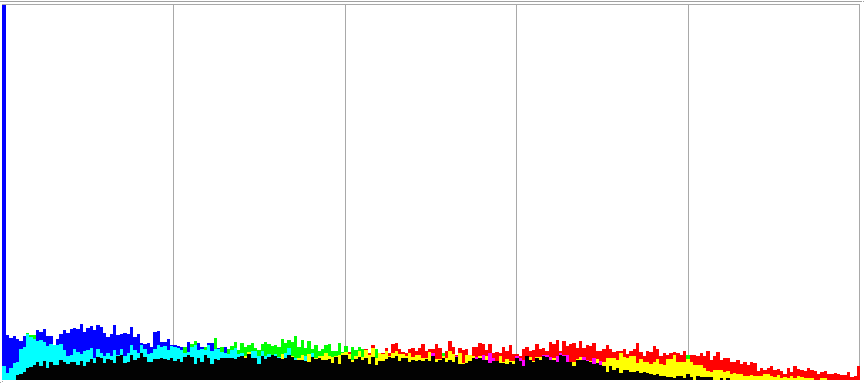
\includegraphics[width=.4\textwidth]{figures/gtOut2Histo.png}}
		\end{center}
		~
		\subfigure[LSB m. besked]{\label{fig:a}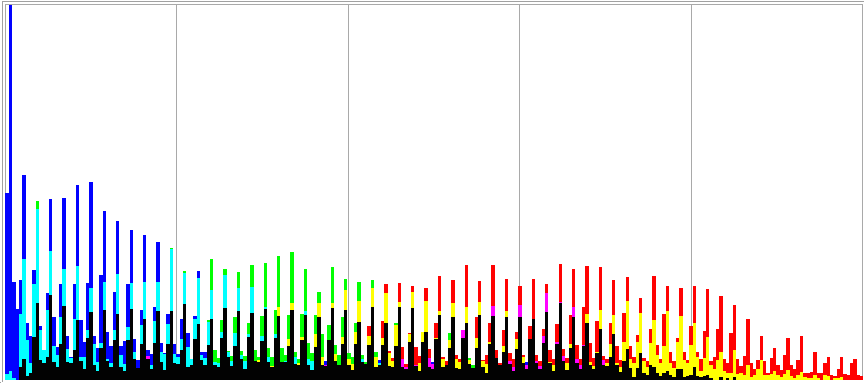
\includegraphics[width=.4\textwidth]{figures/lsbOutHisto.png}}
		~
		\subfigure[GT m. besked]{\label{fig:b}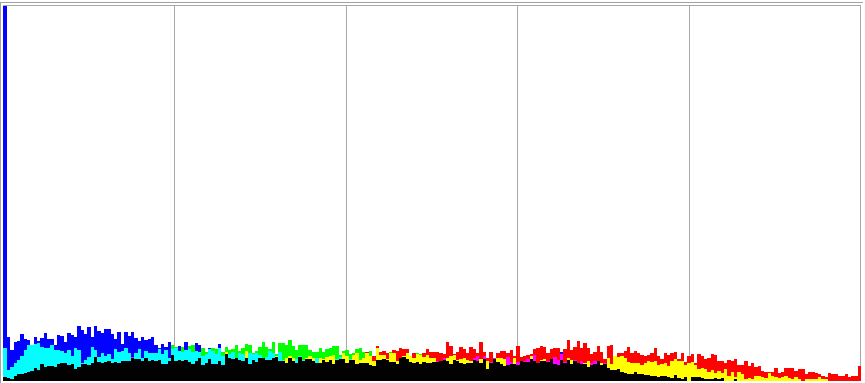
\includegraphics[width=.4\textwidth]{figures/gtOutHisto.png}}
		\caption{Samme besked, forskellige metoder}
	\end{figure}
\end{frame}
